\paragraph{}
Here I will describe in details what each algorithm does

\section{OpenCV}
\subsection{Image Thresholding}
\paragraph{Introduction}
Thresholding is a process of creating binary image from a grayscale one.\cite{digital-image-processing} It is the simplest form of segmentation (separating image into regions). It uses the simplest property that pixels in a region can share - the intensity. Hence thresholding is a natural way of separating light and dark regions of the image. In simple words, all pixels with intensity value below some threshold are being assigned zero and all pixels with intensity above this threshold one. Pixels that are equal the threshold value are treated either as zero or one but the behaviour needs to be consistent. 

\begin{equation}
	g(x, y) = \begin{cases}
		1 & \text{if $f(x, y) >= T$}\\
		0 & \text{otherwise}
	\end{cases}
\end{equation}

\paragraph{Problems with thresholding}
The most significant issue with thresholding is the fact that only the intensity is considered and no relationship between pixels is. This can lead to the inclusion of external pixels that are not part of the original region. Similarly, isolated pixels can be lost from a region. The presence of noise in the image can easily worsen the outcome, because pixels intensity may not represent the normal intensity in the region. The usage of thresholding is often based on experimentation and small adjustments. Still, a large portion of a region may be lost or the area may be extended with extraneous background pixels (especially when shadows of objects are presents - which causes them to be included as part of dark object on a light background). One of the flaws of global image thresholding is also the fact that it is not particularly effective when changes in illumination occur in the image. This drawback can partially be mitigated by determining thresholds locally, so instead of a single global threshold value, the threshold itself can actually vary across different parts of the image.

\todo{Add images that showcase different thresholding}

\begin{figure}[H]
	\centering
	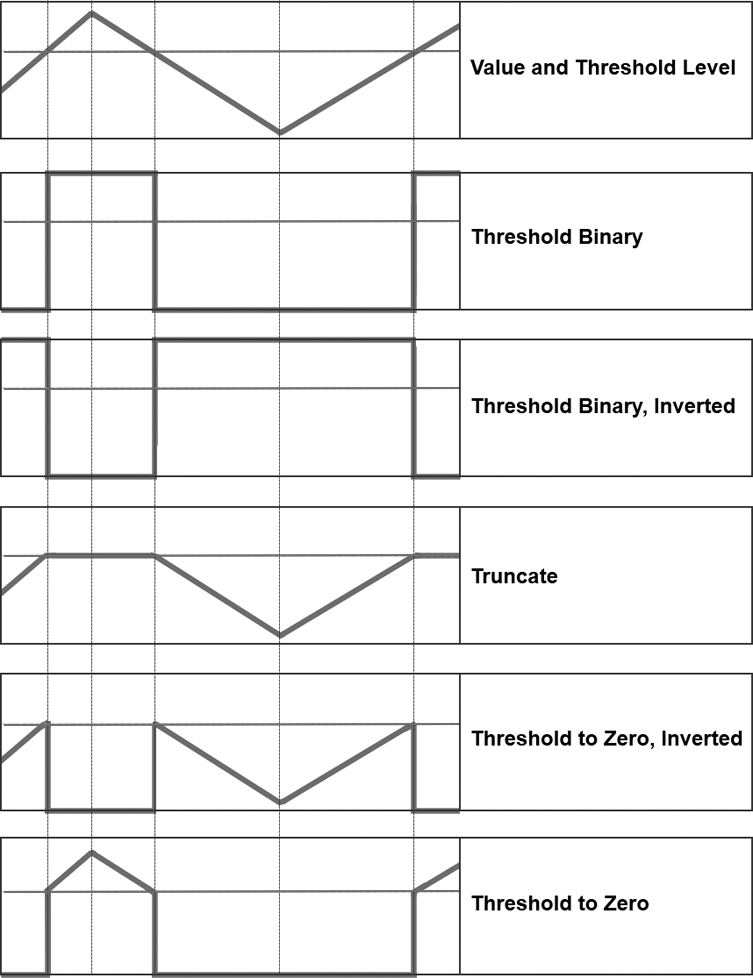
\includegraphics[width=\textwidth]{images/thresholds}
	\caption{Thresholding variants in OpenCV}
\end{figure}

\subsection{Image Filtering}
\paragraph{Introduction}
Filtering is a technique for modifying or enhancing an image. It is used either to emphasize some features of the image or to remove some other. Images can be filtered with various low-pass filters (LPF) or high-pass filters (HPF). HPFs are useful for finding edges in the images whereas LPFs are used to remove noise and for image blurring.

\paragraph{Correlation and convolution}
This are basic operations that can be applied in order to extract information from an image. In a sense they are the simplest operations that can be performed but, nevertheless, extremely powerful and useful. Due to their simplicity they are also well understood, easy implementable and efficiently computable. Both of these operations fullfill two features:
\begin{itemize}
	\item Linearity
	\item Shift-invariance
\end{itemize}
Let us now look at correlation in 2D. Given a square filter with odd number of elements represented by a $(2N + 1)$ x $(2N + 1)$ matrix $F$ and the image matrix $I$, the results of correlation can be computed by aligning the center of the filter with a pixel. Overlapping values are then multiplied together and summed up to make the result corresponding to that given pixel. It can be written as
\begin{equation}
	(F \otimes I)(x, y) = \sum_{i = -N}^{N}\sum_{j = -N}^{N}F(i, j)I(x + i, y + j)
\end{equation}
\todo{Insert example here showing matrices and the operations being applied}
Convolution is very similar to correlation, but the filter is flipped both horizontally and vertically beforehand. 
\begin{equation}
	(F \star I)(x, y) = \sum_{i = -N}^{N}\sum_{j = -N}^{N}F(i, j)I(x - i, y - j)
\end{equation}
The key distinction before the two operations is the associative property of convolution:
\begin{equation}
	\forall F, G - filters \quad \forall I - image: F \star (G \star I) = (F \star G) \star I
\end{equation}
This property is useful when there is need to convolve image with multiple filters. It is computationally faster to precompute the final filter as convolution of original filters and apply just one convolution to the input image. Convolutions are used for image processing operations such as smoothing whereas correlations are useful for matching templates.
One final notice, that for symmetrical filters convolution and correlation are identical.

\paragraph{Image blurring}
To achieve smoothing effect, the image is convolved with a LPF kernel. This particular type of filtering removes high frequency content from the image (for example noise). Unfortunately, edges also can be blurred a bit while applying this operation, although there are also smoothing filters that prevent edges from being blurred. The OpenCV library provides user with various filters amongst which the most popular ones are:
\begin{itemize}
	\item Averaging - it takes the average of all the pixels under kernel area
	\item Gaussian - instead of box filter, a Gaussian kernel is used
	\item Median - in this case the median value of all the pixels under kernel area is used
	\item Bilateral - slower compared to other filters, but it keeps edges sharp
\end{itemize}

\subsection{Morphological Transformations}
\subsection{Finding Contours}
\subsection{Canny Edge Detection}
\subsection{Hough Lines Detection}

\section{Finding the Projection}

\section{Reading the Code}

\section{Comparing Two Codes}